\documentclass[11pt,a4paper]{scrartcl}

\usepackage{fullpage}

%\usepackage[ngerman]{babel}
\usepackage[utf8]{inputenc}
\usepackage{graphicx}

\usepackage{amsmath}
\usepackage{amsfonts}
\usepackage{amsthm}
%\usepackage{mathtools}

\usepackage{listings}

%%%%% COMMANDS

\newcommand{\FT}{\mathcal{F}}
\newcommand{\T}{\mathrm{T}}
\newcommand{\IFT}{\mathcal{F}^{-1}}
\newcommand{\conv}{\ast}
\newcommand{\defined}{\coloneqq}
\newcommand{\IR}{\mathbb{R}}
\newcommand{\IZ}{\mathbb{Z}}
\newcommand{\map}{\rightarrow}


\newtheorem*{theorem}{Theorem}

\renewcommand{\thesubsection}{\alph{subsection})}

\begin{document}

\title{Artificial Intelligence Exercise 2}
\author{Markus Döring, 3153320}
\maketitle

\section{Search Algorithms}
\subsection{Tree Traversal}
See figure \ref{fig:search}.
\begin{figure}[ht]
 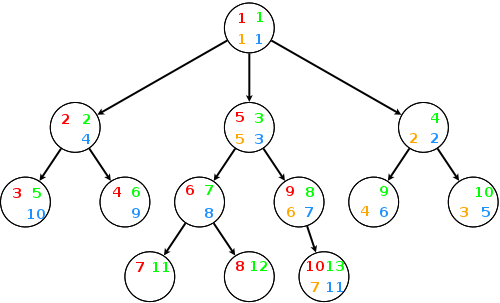
\includegraphics[width=.65\linewidth]{search.png}
 \caption{Tree traversal. The order of node expansion is color coded: For the ``left to right'' types, 
 depth-first is red and breadth-first is green. For the ``right to left'' types, depth-first is orange, 
 breadth-first is blue. The total number of visited nodes can be read at the bottom right target node.}
 \label{fig:search}
\end{figure}

\subsection{Infinite Trees}

If the depth of a search tree is infinite, then depth-first search is in general 
not complete - it can get stuck in one infinite branch while the goal state is 
in another one. Breadth-First search is compelete for trees with infinite depth, 
because all nodes of one layer are visited before the algorithm advances to the 
next layer. Trees with infinite width could be a problem for breadth-first search, 
but such trees would turn out much more problematic in other ways, namely memory 
usage.

\section{Water-Jug Problem}

\subsection{Problem}
We describe states as vectors $s = (x,y)^T\in\IR^2$, with entries $x,y$ representing 
the amount of water in each jug, in liters. The initial state would therefore 
be $(0,0)^T$, and the target state $(0,4)^T$. Path costs can be chosen constant 
(e.g., $c=1$). An action $f:\ \IR^2\map\IR^2,$ is valid if

\begin{itemize}
\item $f(x,y) = (0,y)^T$ or
\item $f(x,y) = (x,0)^T$ or 
\item $f(x,y) = (\min(\{3, x+y\}), y-\min(\{3-x,y\}))^T$ or
\item $f(x,y) = (x-\min(\{5-y,x\}), \min(\{5,x+y\}))^T$.
\end{itemize}

\subsection{State-Space Graph}
See figure \ref{fig:water}.
\begin{figure}[ht]
 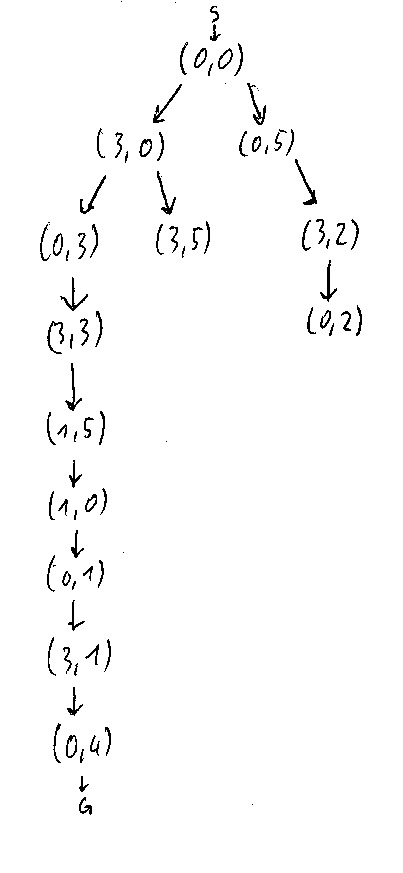
\includegraphics[width=.35\linewidth]{water_red.jpg}
 \caption{The state space graph of the water jug problem, ignoring edges that lead to cycles.}
 \label{fig:water}
\end{figure}

\subsection{}
I'm not going to draw any more state spaces (or trees, for that matter), but I promise I know how to traverse a tree.

\section{Missionaries and Cannibals}

See the python script \verb$mcb.py$. 

\section{Optimality of $A^*$}

\begin{theorem}
Let $h$ be an admissible heuristic function, that is for all nodes $n$ and for the 
true cost function $h^*$ 
\begin{equation*}
h(n)\leq h^*(n)
\end{equation*}
holds. Then the $A^*$ algorithm is optimal on every search tree $T$.
\end{theorem}
\begin{proof}
Let $f(n) = g(n) + h(n)$ denote the cost estimate function that $A^*$ tries to 
minimize. The function $g$ gives the true cost up to node $n$, and $h$ is the 
heuristic for the cost from state $n$ to a goal state. Let $P_m, P_n$ be to paths which lead to goal states 
$G_m, G_n$, respectively, and let $P_m$ be more expensive than $P_n$.

We prove the theorem indirectly. Choose $m$ as the adjacent node of $G_m$ on $P_m$, and assume that $G_m$ is accepted 
as a solution by the algorithm. Then there is a first node $n$ on $P_n$ which has not been expanded such that
\begin{equation*}
f(G_m) = g(m) + h^*(m) \leq g(n) + h(n) = f(n) .
\end{equation*}
$P_n$ is shorter than $P_m$, which implies
\begin{equation*}
g(G_n) = g(n) + h^*(n) < g(m) + h^*(m) = g(G_M),
\end{equation*}
and chaining the inequalities results in 
\begin{equation*}
g(n) + h^*(n) < g(n) + h(n),
\end{equation*}
which contradicts the admissability of $h$. Therefore, all nodes on path $P_n$ get expanded before $G_m$ is acccepted, 
and the optimal path is found.
\end{proof}
%\newpage
%\appendix
%\lstinputlisting[language=python]{ia_05_01.py}
%\newpage
%\lstinputlisting[language=python]{ia_05_02.py}
\end{document}
